% !TEX encoding = UTF-8 Unicode
\documentclass[a4paper]{article}

\usepackage{lipsum}
\usepackage{tcolorbox}
\usepackage{color}
\usepackage{url}
%\usepackage[T2A]{fontenc} % enable Cyrillic fonts
\usepackage[utf8]{inputenc} % make weird characters work
\usepackage{graphicx}
\usepackage{amsmath}
%\usepackage[obeyspaces]{url}
\usepackage[T1]{fontenc}
% \usepackage{inconsolata}

\usepackage[english,serbian]{babel}
%\usepackage[english,serbianc]{babel} %ukljuciti babel sa ovim opcijama, umesto gornjim, ukoliko se koristi cirilica

\usepackage[german=quotes]{csquotes}
\DeclareQuoteAlias{ngerman}{serbian}
\MakeOuterQuote{"}

\usepackage[unicode]{hyperref}
\hypersetup{colorlinks,citecolor=green,filecolor=green,linkcolor=blue,urlcolor=blue}

\usepackage{epigraph}

%\renewcommand{\epigraphflush}{center}
%\setlength{\epigraphwidth}{0.8\textwidth}
%\renewcommand{\textflush}{flushepinormal}
%\setlength{\epigraphrule}{0pt}

\usepackage{listings}

%\newtheorem{primer}{Пример}[section] %ćirilični primer
\newtheorem{primer}{Primer}[section]

\definecolor{mygreen}{rgb}{0,0.6,0}
\definecolor{mygray}{rgb}{0.5,0.5,0.5}
\definecolor{mymauve}{rgb}{0.58,0,0.82}

\lstdefinelanguage{Clojure}%
{morekeywords={*,*1,*2,*3,*agent*,*allow-unresolved-vars*,*assert*,*clojure-version*,*command-line-args*,%
*compile-files*,*compile-path*,*e,*err*,*file*,*flush-on-newline*,*in*,*macro-meta*,%
*math-context*,*ns*,*out*,*print-dup*,*print-length*,*print-level*,*print-meta*,*print-readably*,%
*read-eval*,*source-path*,*use-context-classloader*,*warn-on-reflection*,+,-,->,->>,..,/,:else,%
<,<=,=,==,>,>=,@,accessor,aclone,add-classpath,add-watch,agent,agent-errors,aget,alength,alias,%
all-ns,alter,alter-meta!,alter-var-root,amap,ancestors,and,apply,areduce,array-map,aset,%
aset-boolean,aset-byte,aset-char,aset-double,aset-float,aset-int,aset-long,aset-short,assert,%
assoc,assoc!,assoc-in,associative?,atom,await,await-for,await1,bases,bean,bigdec,bigint,binding,%
bit-and,bit-and-not,bit-clear,bit-flip,bit-not,bit-or,bit-set,bit-shift-left,bit-shift-right,%
bit-test,bit-xor,boolean,boolean-array,booleans,bound-fn,bound-fn*,butlast,byte,byte-array,%
bytes,cast,char,char-array,char-escape-string,char-name-string,char?,chars,chunk,chunk-append,%
chunk-buffer,chunk-cons,chunk-first,chunk-next,chunk-rest,chunked-seq?,class,class?,%
clear-agent-errors,clojure-version,coll?,comment,commute,comp,comparator,compare,compare-and-set!,%
compile,complement,concat,cond,condp,conj,conj!,cons,constantly,construct-proxy,contains?,count,%
counted?,create-ns,create-struct,cycle,dec,decimal?,declare,def,definline,defmacro,defmethod,%
defmulti,defn,defn-,defonce,defprotocol,defstruct,deftype,delay,delay?,deliver,deref,derive,%
descendants,destructure,disj,disj!,dissoc,dissoc!,distinct,distinct?,do,do-template,doall,doc,%
dorun,doseq,dosync,dotimes,doto,double,double-array,doubles,drop,drop-last,drop-while,empty,empty?,%
ensure,enumeration-seq,eval,even?,every?,false,false?,ffirst,file-seq,filter,finally,find,find-doc,%
find-ns,find-var,first,float,float-array,float?,floats,flush,fn,fn?,fnext,for,force,format,future,%
future-call,future-cancel,future-cancelled?,future-done?,future?,gen-class,gen-interface,gensym,%
get,get-in,get-method,get-proxy-class,get-thread-bindings,get-validator,hash,hash-map,hash-set,%
identical?,identity,if,if-let,if-not,ifn?,import,in-ns,inc,init-proxy,instance?,int,int-array,%
integer?,interleave,intern,interpose,into,into-array,ints,io!,isa?,iterate,iterator-seq,juxt,%
key,keys,keyword,keyword?,last,lazy-cat,lazy-seq,let,letfn,line-seq,list,list*,list?,load,load-file,%
load-reader,load-string,loaded-libs,locking,long,long-array,longs,loop,macroexpand,macroexpand-1,%
make-array,make-hierarchy,map,map?,mapcat,max,max-key,memfn,memoize,merge,merge-with,meta,%
method-sig,methods,min,min-key,mod,monitor-enter,monitor-exit,name,namespace,neg?,new,newline,%
next,nfirst,nil,nil?,nnext,not,not-any?,not-empty,not-every?,not=,ns,ns-aliases,ns-imports,%
ns-interns,ns-map,ns-name,ns-publics,ns-refers,ns-resolve,ns-unalias,ns-unmap,nth,nthnext,num,%
number?,odd?,or,parents,partial,partition,pcalls,peek,persistent!,pmap,pop,pop!,pop-thread-bindings,%
pos?,pr,pr-str,prefer-method,prefers,primitives-classnames,print,print-ctor,print-doc,print-dup,%
print-method,print-namespace-doc,print-simple,print-special-doc,print-str,printf,println,println-str,%
prn,prn-str,promise,proxy,proxy-call-with-super,proxy-mappings,proxy-name,proxy-super,%
push-thread-bindings,pvalues,quot,rand,rand-int,range,ratio?,rational?,rationalize,re-find,%
re-groups,re-matcher,re-matches,re-pattern,re-seq,read,read-line,read-string,recur,reduce,ref,%
ref-history-count,ref-max-history,ref-min-history,ref-set,refer,refer-clojure,reify,%
release-pending-sends,rem,remove,remove-method,remove-ns,remove-watch,repeat,repeatedly,%
replace,replicate,require,reset!,reset-meta!,resolve,rest,resultset-seq,reverse,reversible?,%
rseq,rsubseq,second,select-keys,send,send-off,seq,seq?,seque,sequence,sequential?,set,set!,%
set-validator!,set?,short,short-array,shorts,shutdown-agents,slurp,some,sort,sort-by,sorted-map,%
sorted-map-by,sorted-set,sorted-set-by,sorted?,special-form-anchor,special-symbol?,split-at,%
split-with,str,stream?,string?,struct,struct-map,subs,subseq,subvec,supers,swap!,symbol,symbol?,%
sync,syntax-symbol-anchor,take,take-last,take-nth,take-while,test,the-ns,throw,time,to-array,%
to-array-2d,trampoline,transient,tree-seq,true,true?,try,type,unchecked-add,unchecked-dec,%
unchecked-divide,unchecked-inc,unchecked-multiply,unchecked-negate,unchecked-remainder,%
unchecked-subtract,underive,unquote,unquote-splicing,update-in,update-proxy,use,val,vals,%
var,var-get,var-set,var?,vary-meta,vec,vector,vector?,when,when-first,when-let,when-not,%
while,with-bindings,with-bindings*,with-in-str,with-loading-context,with-local-vars,%
with-meta,with-open,with-out-str,with-precision,xml-seq,zero?,zipmap
},%
   sensitive,% ???
   alsodigit=-,%
   morecomment=[l];,%
   morestring=[b]"%
  }[keywords,comments,strings]%
  

\lstset{ 
  backgroundcolor=\color{white},   % choose the background color; you must add \usepackage{color} or \usepackage{xcolor}; should come as last argument
  basicstyle=\scriptsize\ttfamily,        % the size of the fonts that are used for the code
  breakatwhitespace=false,         % sets if automatic breaks should only happen at whitespace
  breaklines=true,                 % sets automatic line breaking
  captionpos=b,                    % sets the caption-position to bottom
  commentstyle=\color{mygreen},    % comment style
  deletekeywords={...},            % if you want to delete keywords from the given language
  escapeinside={\%*}{*)},          % if you want to add LaTeX within your code
  extendedchars=true,              % lets you use non-ASCII characters; for 8-bits encodings only, does not work with UTF-8
  firstnumber=1000,                % start line enumeration with line 1000
  frame=single,	                   % adds a frame around the code
  keepspaces=true,                 % keeps spaces in text, useful for keeping indentation of code (possibly needs columns=flexible)
  keywordstyle=\color{blue},       % keyword style
  language=Clojure,                 % the language of the code
  morekeywords={*,...},            % if you want to add more keywords to the set
  numbers=left,                    % where to put the line-numbers; possible values are (none, left, right)
  numbersep=5pt,                   % how far the line-numbers are from the code
  numberstyle=\tiny\color{mygray}, % the style that is used for the line-numbers
  rulecolor=\color{black},         % if not set, the frame-color may be changed on line-breaks within not-black text (e.g. comments (green here))
  showspaces=false,                % show spaces everywhere adding particular underscores; it overrides 'showstringspaces'
  showstringspaces=false,          % underline spaces within strings only
  showtabs=false,                  % show tabs within strings adding particular underscores
  stepnumber=2,                    % the step between two line-numbers. If it's 1, each line will be numbered
  stringstyle=\color{mymauve},     % string literal style
  tabsize=2,	                   % sets default tabsize to 2 spaces
  title=\lstname                   % show the filename of files included with \lstinputlisting; also try caption instead of title
}

\begin{document}

\title{Otvoreno o Zatvorenju\\ \small{Seminarski rad u okviru kursa\\Metodologija stručnog i naučnog rada\\ Matematički fakultet}}

\author{N. Grulović, J. Dmitrović, D. Martinović, N. Bogdanović\\ \small{n.grulovic@outlook.com, jdmitrovic@gmail.com, dunavpe@gmail.com, nadezdabogdanovic1@gmail.com}}

\date{6.april 2019.}

\maketitle

\abstract{
Clojure (\textit{zatvorenje}) je dinamičan, homoikoničan jezik opšte namene, sa naglaskom na funkcionalnom programiranju. Poslednjih godina, može se primetiti sve veći broj korisnika i pristalica Clojure-a, što ne čudi, imajući u vidu nagli porast u popularnosti funkcionalnih jezika. Cilj ovog rada je da približi čitaocu ovaj programski jezik i ukaže mu na oblasti, kao i načine njegove primene.}

\tableofcontents

\newpage

% _________________Sekcije_______________________

\section{Uvod}
\label{sec:uvod}

\epigraph{"Bolje je imati 100 funkcija koje operišu nad jednom strukturom podataka, nego 10 funkcija koje operišu nad 10 različitih struktura podataka."}{\textit{ --- Alan J. Perlis}}

 Kao savremeni dijalekt Lisp programskog jezika, čiji makro-sistem poseduje, Clojure posmatra kod kao podatke nepromenljive strukture. Uspešno kombinuje pristupačnost i interaktivan razvoj, kakav se može susresti kod skriptnog jezika, sa efikasnom i robustnom infrastrukturom višenitnog programiranja.
 
 Uprkos činjenici da je kao jezik kompajliran, on uspeva da očuva potpunu dinamičnost i time omogući da svaka osobenost podržana od strane Clojure-a bude podržana i za vreme izvršavanja. Njegov osnovni interfejs za programiranje, REPL, nas oslobađa ograničenja u smislu kompajliranja i pokretanja izvršnog koda kao jedinih opcija i daje slobodu interaktivnog pisanja programa.

Kao mlad jezik, Clojure je ređe korišćen, ako ne i slabije poznat u programerskim krugovima, uprkos velikim mogućnostima koje pruža. Često je okarakterisan, od strane svojih pristalica, kao zabavan jezik koji dopušta drugačiji pogled na samu logiku programiranja.

Ono što čini Clojure veoma omiljenim i pristupačnim, jeste veliki dijapazon šablona i modularnih biblioteka. Posedujući visok stepen unapred definisane modularnosti, on omogućava da se projekat započne odmah, a istovremeno onemoguće moduli od kojih nema trenutne koristi, čime rezultuje niskom potrošnjom resursa i visokom efikasnošću implementacije.

U ovom radu, čitaocu će najpre biti predstavljena osnovna svojstva jezika i pojašnjenja njegove sintakse, a zatim će, vođen uputstvom za instalaciju i primerom koda biti u mogućnosti da se i sam okuša u programiranju.

\newpage

\section{Razvoj programskog jezika Clojure}
\label{sec:razvoj}

Clojure je razvijen od strane Riča Hikija(engl. \textit{Rich Hickey})\cite{clojure}, tvorca .Lisp-a i drugih Lisp-olikih jezika, pokušaja povezivanja sa Javom. Prva verzija je zvanično objavljena 16.10.2007. iako je jezik postojao već dve godine. U tabeli \ref{tab:verzije}, hronološki su predstavljene sve objavljene verzije i njihove glavne odlike.

\begin{table}[h!]
\begin{center}
\begin{tabular}{|c|c|c|} \hline
\textbf{Verzija} & \textbf{Datum izlaska} & \textbf{Novine}\\ \hline
 & 16.10.2007. & Prvo zvanično objavljivanje \\ \hline
1.0 & 04.05.2009. & Prva stabilna verzija\\ \hline
1.1 & 31.12.2009. & Operator \texttt{future} za sinhronizaciju\\ \hline
1.2 & 19.08.2010. & Protokoli\\ \hline
1.3 & 23.09.2011. & Napredna podrška za primitive\\ \hline
1.4 & 15.04.2012. & Literali čitača\\ \hline
1.5 & 01.03.2013. & Reduktori\\ \hline
1.6 & 25.03.2014. & Java API, unapređeni heš algoritmi\\ \hline
1.7 & 30.06.2015. & Uslovi za čitač, transduktori\\ \hline
1.8 & 19.01.2016. & Funkcije za niske, direktno linkovanje\\ \hline
1.9 & 08.12.2017. & Alati komandne linije\\ \hline
\textbf{1.10} & 17.12.2018. & Izveštaji o greškama, Java kompatibilnost\\ \hline
\end{tabular}
\caption{Objavljene verzije\cite{clojure_release_1}\cite{clojure_release_2}\cite{clojure}}
\label{tab:verzije}
\end{center}
\end{table}

Razvoju jezika umnogome je doprinela njegova zajednica, koja je aktivna od trenutka kada se on pojavio. Clojure konferencije, od kojih su najposećenije one u Sjedinjenim državama i evropske konferencije, organizuju se svake godine širom planete.

\subsection{Odnos sa drugim programskim jezicima}
\label{subsec:drugijezici}

Kao odgovor na pitanje zašto je osmislio još jedan Lisp-oliki jezik, njegov tvorac je odgovorio: "U osnovi, bio mi je potreban Lisp za funkcionalno programiranje, simbiotičan sa osnovnom Java platformom i dizajniran za konkurentnost. Nisam mogao da pronađem takav jezik, pa sam ga stvorio"\cite{clojure}.


 \begin{figure}[h]
     % 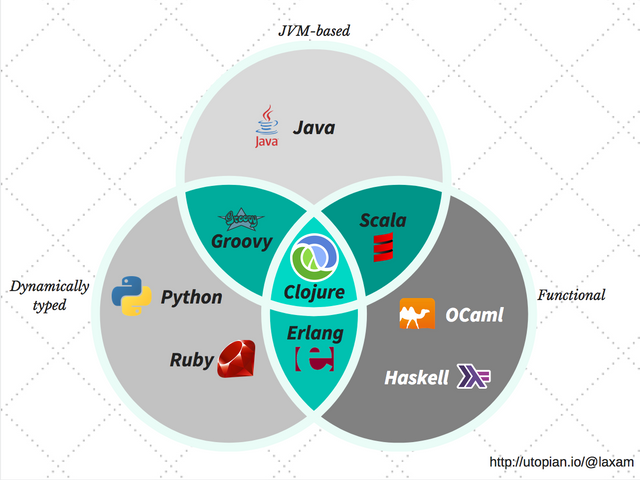
\includegraphics[width=0.6\textwidth]{Slike/clojure.png}
     \centering
     % \hspace{2.5cm}
     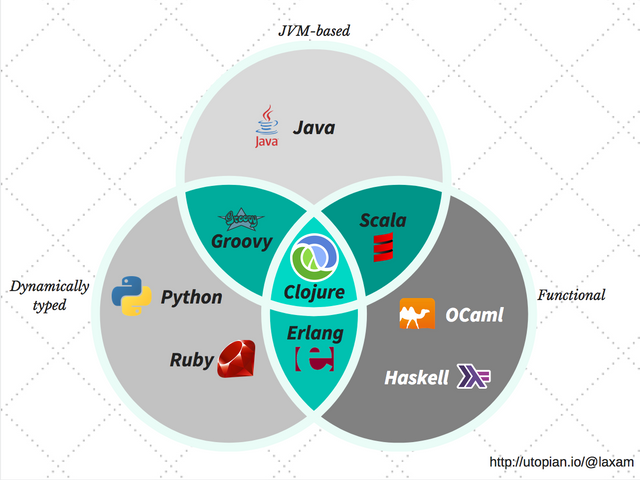
\includegraphics[width=0.5\textwidth]{Slike/clojure.png}
     \caption{Odnos Clojure-a i drugih programskih jezika\cite{diagram}}
     \label{fig:clojure_ostali}
 \end{figure}

Kao direktan Lisp-ov potomak, smestio se u stablu \ref{fig:stablo} programskih jezika  kao "mlađi brat" funkcionalnih jezika kao što su ML, Smalltalk i Dylan.

\begin{figure}[ht]
    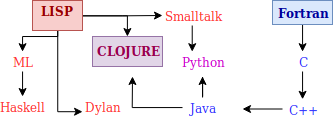
\includegraphics[width=0.6\textwidth]{Slike/stablo2.png}
    \centering
    \caption{Clojure u stablu programskih jezika}
    \label{fig:stablo}
\end{figure}

\section{Osnovna svojstva}
\label{sec:osnovnasvojstva}

Clojure je dijalekat programskog jezika Lisp. Drugim rečima, oba jezika počivaju na istim postulatima. U saglasnosti sa tim, Clojure je, pre svega, funkcionalni programski jezik, a pored toga, ima bliskosti i sa konkurentnom i reaktivnom paradigmom\cite{clojure}.

\subsection{Platforme}
\label{subsec:platforme}

Budući da je Clojure funkcionalni programski jezik, njegova veza sa programskim jezikom Java, koji je predstavnik objektno-orijentisane paradigme, može biti iznenađujuća. Clojure je dizajniran tako da bude tzv. \textit{hosted} programski jezik - za razliku od jezika kao što su C, Python ili Haskell koji prevode svoj izvorni kôd u mašinski ili međukod, Clojure prevodi izvorni kôd u Java bajtkod koji će se potom izvršavati uz pomoć Java Virtuelne Mašine (engl. \textit{Java Virtual Machine}). JVM je izabrana kao standardna platforma za Clojure zbog svoje portabilnosti, sigurnosti, kao i rasprostranjenosti u industriji.


Kako poslednjih godina raste naklonost ka funkcionalnim jezicima, tako raste i broj platformi kompatibilnih sa ovim jezikom. Neke od implementacija koje koriste alternativne platforme su ClojureScript \cite{clojure_script}, ClojureCLR\cite{clojure_clr}, clojure-py\cite{clojure_py} omogućava integraciju sa Pythonom, Ferret\cite{ferret} sa C++, clojerl\cite{clojerl} sa Erlangom i Joker\cite{joker} interpreter i linter pisan u programskom jeziku Go.


\subsection{Clojure kao funkcionalni programski jezik}
\label{subsec:funkcionalni}

Kao i u svim funkcionalnim jezicima, u Clojure-u se funkcije posmatraju kao \emph{građani prvog reda}; drugim rečima, ne postoji ograničenje kako se funkcije mogu kreirati ili koristiti. Međutim, Clojure nije \emph{čist} funkcionalni jezik, tako da se ne drži strogih pravila o referencijalnoj transparentnosti\cite{transparency_2}\cite{transparency}.

Jedna od karakteristika koju Clojure deli sa programskim jezikom Lisp jeste \textbf{homoikoničnost} (engl. \textit{homoiconicity}). Izvorni kôd homoikoničnih programskih jezika se posmatra kao struktura podataka napisanog u tom istom programskom jeziku. Ovo svojstvo omogućava programima napisanim u Clojure-u da manipulišu drugim Clojure programima, kao i da ih generišu.

Raspolažući samo sa imutabilnim objektima, Clojure na taj način rešava probleme koje donosi mutabilnost objekata. Budući da to rešenje doprinosi činjenici da se narušavaju performanse nekih operacija na strukturama podataka kao što su vektori i heš mape, te strukture su interno implementirane uz pomoć heš stabala.

Kako lokalne promenljive ne postoje u Clojure-u, petlje se emuliraju uz pomoć (repne) rekurzije. Mnogi funkcionalni programski jezici omogućavaju da repna rekurzija ne koristi stek okvire, time održavajući konstantnu prostornu složenost rekurzivnih poziva; Clojure nema tu mogućnost, zbog načina na koji JVM poziva funkcije. Ovaj problem se prevazilazi korišćenjem operatora \texttt{recur}\cite{livingclojure}.

\subsection{Dinamičko programiranje}
\label{subsec:dinamickoprogramiranje}

Prilikom programiranja u programskom jeziku Clojure, nismo ograničeni samo na kompajliranje i pokretanje izvršnog kôda - postoji i mogućnost interaktivnog pisanja programa.
Iako se Clojure može ugraditi u Java kôd, osnovni interfejs za programiranje predstavlja \textbf{REPL} (\textit{\textbf{R}ead-\textbf{E}val-\textbf{P}rint-\textbf{L}oop}). REPL je konzolni interfejs gde se napisani Clojure kôd evaluira za svaku napisanu liniju. Ovakav pristup programiranju daje brz odziv na promene u programu što čini neke zadatke jednostavnijim, na primer pronalaženje i uklanjanje bagova. 

\section{Instalacija}
\label{sec:instalacija}
Clojure pruža skup alata komandne linije koji se mogu koristiti za pokretanje Clojure REPL-a, upotrebu Java i Clojure biblioteka i pokretanje Clojure programa.
\subsection{Linux}
\label{subsec:linux}
\begin{enumerate}
            \item Obezbediti da su instalirani paketi: \texttt{curl}, \texttt{rlwrap}, i \texttt{java}.
            Provera verzija pomenutih paketa se vrši putem komandi:
            \begin{tcolorbox}[colback=green!5!white,colframe=green!5!white,fontupper=\ttfamily]
            \$ curl -V \newline
            \$ rlwrap -v \newline
            \$ java -version
            \end{tcolorbox}
            Instalacija:
            \begin{tcolorbox}[colback=green!5!white,colframe=green!5!white,fontupper=\ttfamily]
            \$ sudo apt install curl \newline
            \$ sudo apt install rlwrap
            \end{tcolorbox}
            Ako nije instalirana Java:
            \begin{tcolorbox}[colback=green!5!white,colframe=green!5!white,fontupper=\ttfamily]
            \$ sudo apt install default-jre \newline
            \$ sudo apt install openjdk-11-jdk
            \end{tcolorbox}
            \item Preuzeti i instalirati pomoću linux skripta za instalaciju, koji će kreirati fajlove /usr/local/bin/clj, /usr/local/bin/clojure, and /usr/local/lib/clojure:
\begin{tcolorbox}[colback=green!5!white,colframe=green!5!white,fontupper=\ttfamily]

\$ curl -O https://download.clojure.org/\\install/linux-install-1.10.0.442.sh

\$ chmod +x linux-install-1.10.0.442.sh

\$ sudo ./linux-install-1.10.0.442.sh
\end{tcolorbox}

\end{enumerate}

\subsection{Windows}
\label{subsec:windows}
Trenutno postoji samo alfa verzija Clojure-a za Windows. Najpre se sa \href{https://github.com/clojure/tools.deps.alpha/wiki/clj-on-Windows}{link-a} preuzme poslednja verzija instalacionog fajla. Nakon pokretanja instalacije, biće ponuđene 3 moguće lokacije za instalaciju:\newline
\begin{tcolorbox}[colback=green!5!white,colframe=green!5!white,fontupper=\ttfamily]
Possible install locations:\newline
  1) \path{\\Drive\Home\Documents\WindowsPowerShell\Modules}\\
  2) \path{C:\Program Files\WindowsPowerShell\Modules}\\
  3) \path{C:\WINDOWS\system32\WindowsPowerShell\v1.0\Modules\ }\\
Enter number of preferred install location: 
\end{tcolorbox}
Treba imati u vidu da pri izboru 1. opcije nisu potrebne admin privilegije, ali se kreira dodatni fajl u \path{\Documents}, dok za 2. i 3. opciju je potrebno imati admin privilegije.

\subsection{Pokretanje}
\label{subsec:pokretanje}
Nakon preuzimanja i instalacije potrebnih alata, REPL se pokreće pomoću komande \texttt{clj}:
\begin{tcolorbox}[colback=green!5!white,colframe=green!5!white,fontupper=\ttfamily]
\$ clj\\
Clojure 1.10.0\\
user=>
\end{tcolorbox}

Prilikom ulaska u REPL, moguće je kucati Clojure izraze i pokretati ih pritiskom na Enter.
Postoji veliki broj Clojure i Java biblioteka koje nude razne funkcionalnosti. Često korišćena biblioteka je \href{https://github.com/clj-time/clj-time}{clj-time} koja radi sa datumima i vremenom.


Da bi se koristila ova biblioteka potrebno je napraviti \textbf{deps.edn} fajl za deklarisanje zavisnosti:
\begin{tcolorbox}[colback=green!5!white,colframe=green!5!white,fontupper=\ttfamily]
\{:deps


\hspace*{5mm}\{clj-time \{:mvn/version ''0.14.2''\}\}\}
\end{tcolorbox}
Za pisanje programa, potrebno je napraviti novi direktorijum i kopirati \textbf{deps.edn} fajl u odgovarajući direktorijum.

Komanda \texttt{clj} automatski traži izvorne fajlove u \textbf{src} direktorijumu pa je potrebno fajl sa ekstenzijom \underline{\textit{.clj}} sačuvati na putanji \path{\src\program.clj} i pokrenuti:

\begin{tcolorbox}[colback=green!5!white,colframe=green!5!white,fontupper=\ttfamily]
\$ clj -m program
\end{tcolorbox}
%\subsubsection{Clojure online}
 
%\subsubsection{Lokalno građenje}
%Clojure je moguće graditi lokalno (neophodni su paketi \texttt{git}, \texttt{java} i \texttt{maven}):
%\begin{tcolorbox}[colback=green!5!white,colframe=green!5!white,fontupper=\ttfamily]
%    \$ git clone https://github.com/clojure/clojure.git\newline
%    \$ cd clojure\newline
%    \$ mvn -Plocal -Dmaven.test.skip=true package
%\end{tcolorbox}
%Pokretanje REPL pomoću lokalnog jar-a:
%\begin{tcolorbox}[colback=green!5!white,colframe=green!5!white,fontupper=\ttfamily]
%    java -jar clojure.jar
%\end{tcolorbox}

Pored instalacije na lokalnom računaru, REPL je moguće koristiti i u web pregledaču pomoću servisa \href{https://repl.it/languages/clojure}{repl.it}. Ova web stranica omogućuje korišćenje više nezavisnih REPL interfejsa, kao i povezivanje sa Github nalogom.

\section{Sintaksna struktura}
\label{sec:sintaksnastruktura}

Kako je Clojure dijalekat programskog jezika Lisp, i sintaksa ta dva jezika je slična. Ono što je karakteristično za ovakve jezike jeste njihova sintaksna \emph{uniformnost}.

\subsection{Literali i operatori}
\label{subsec:literalioperatori}

\lstinputlisting[language=Clojure, caption={Literali},frame=single, label=literali]{Kodovi/literali.clj}

\textbf{Literali} su najjednostavniji izrazi - to su oni izrazi koji se evaluiraju u sami sebe. Neki od osnovnih literala u programskom jeziku Clojure su:

\begin{itemize}
    \item Celi brojevi
    \item Brojevi u pokretnom zarezu
    \item Razlomljeni brojevi
    \item Niske
    \item Ključne reči
\end{itemize}

Brojevi se predstavljaju na način koji je standardan u programskim jezicima, niske se predstavljaju sa dvostrukim navodnicima (jednostruki nisu dozvoljeni), dok su ključne reči obeležene sa dvotačkom ispred reči (ali reč je navedena \emph{bez} navodnika).
Ključne reči se koriste za referisanje, na primer prilikom dohvatanja elemenata mape.

Literali se koriste zajedno uz pomoć \textbf{operatora} - ugrađenih funkcija. Korišćenje operatora (i drugih definisanih funkcija) se obavlja na sledeći način:

\begin{verbatim}
(operator operand_1 operand_2)
\end{verbatim}

Opisan je binarni, ali se na analogan način koristi i n-arni operator. Primetimo da su zagrade \emph{obavezne}, kao i da se operandi razdvajaju blanko karakterom (zapeta se takođe smatra blanko karakterom). Neki od operatora su dati u narednom listingu:

\lstinputlisting[language=Clojure, caption={Aritmetički, relacioni i logički operatori},frame=single, label=operatori]{Kodovi/operatori.clj}

Operator \texttt{/} se različito ponaša u zavisnosti od operanada: ukoliko su oba operanda celi brojevi, onda je rezultat izračunavanja tog izraza razlomljeni broj ili ceo broj (ako je prvi operand deljiv drugim). Ukoliko je neki od operanada broj u pokretnom zarezu, onda je i rezultat broj u pokretnom zarezu.

Dodeljivanje imena vrednostima se vrši pomoću operatora \texttt{def}:

\begin{verbatim}
(def ime_konstante operand_1)
\end{verbatim}

U drugim programskim jezicima, vrednosti se dodeljuju promenljivama. To nije slučaj u Clojure-u, zbog njegove imutabilne prirode.

\subsection{Kontrola toka}
\label{subsec:kontrolatoka}

U Clojure-u nisu izostali mehanizmi kontrole toka. Za naredbu grananja, koristi se operator \texttt{if}:

\lstinputlisting[language=Clojure, caption={Operatori \texttt{if} i \texttt{do}},frame=single, label=operator_if]{Kodovi/operator_if.clj}

Operator \texttt{if}, ukoliko je vrednost prvog operanda \texttt{true} vraća vrednost drugog operanda; inače, vraća vrednost trećeg operanda. Else grana u okviru operatora \texttt{if} nije obavezna.

Treba napomenuti da se sve vrednosti tretiraju kao tačne, osim literala \texttt{nil} i \texttt{false}. Operator \texttt{and} vraća poslednju tačnu vrednost ukoliko su svi operandi tačni; inače vraća prvu netačnu vrednost. Analogno, operator \texttt{or} vraća poslednju netačnu vrednost ukoliko su svi operandi netačni; inače, vraća se vrednost prvog tačnog operanda.

Operator \texttt{do} omogućava da se izvrši više operacija u nekoj ili obe grane. Povratna vrednost ovog operatora je vrednost poslednjeg operanda.

\subsection{Definisanje funkcija}
\label{subsec:definisanjefja}

Korišćenje funkcija je identično korišćenju operatora. Njihovo definisanje se vrši pomoću operatora \texttt{defn} sledeći način:

\lstinputlisting[language=Clojure, caption={Definisanje funkcija sa tačnim i proizvoljnim brojem parametara},frame=single, label=funkcije]{Kodovi/def_funkcija.clj}

Prvi operand je ime funkcije (navodi se \emph{bez} navodnika), zatim (opciono) postavljanje deskripcije koja se može dohvatiti operatorom \texttt{doc}, treći operand je vektor koji sadrži argumente funkcije i, na kraju, povratna vrednost funkcije.

Primetimo da je moguće definisati funkciju tako da uzima proizvoljan broj parametara; to se postiže korišćenjem simbola \texttt{\&} koji će poslate parametre smestiti u listu.

\subsection{Strukture podataka}
\label{strukturepodataka}

U Clojure-u je dostupno korišćenje tradicionalnih struktura podataka kao što su liste, vektori, mape i skupovi.  Treba napomenuti da elementi ovih struktura podataka ne moraju biti istog tipa.

Liste su definisane na sledeći način:

\begin{verbatim}
'(element_1 element_2 element_3)
\end{verbatim}

Na sličan način se definišu i vektori, ali se koriste simboli \texttt{[} i \texttt{]}. Operatorom \texttt{nth} se može dohvatiti n-ti element liste, dok se ista stvar za vektore postiže korišćenjem operatora \texttt{get}. Dodavanje novih elemenata u listu ili vektor se vrši pomoću operatora \texttt{conj}; novi element će biti dodat na početak liste, odnosno na kraj vektora.

Mape se definišu ili putem operatora \texttt{hash-map} ili uz pomoć vitičastih zagrada:

\begin{verbatim}
{:prva_kljucna_rec vrednost_1 :druga_kljucna_rec vrednost_2}
\end{verbatim}

Pomenuti \texttt{get} operator će vratiti vrednost navedene ključne reči.

Skupovi su vektori čiji su svi elementi jedinstveni. Njihova definicija je:

\begin{verbatim}
#{element_1 element_2 element_3}
\end{verbatim}

Naknadna pojavljivanja istih elemenata u okviru istog skupa biće ignorisana. Za proveru pripadnosti neke vrednosti skupu koristi se operator \texttt{contains?}.

\section{Framework}
\label{sec:framework}
Ono što čini Clojure atraktivnim je veliki spektar šablona i modularnih biblioteka. Dovoljno je univerzalan da radi na gotovo svakom JVM-u, dok je dinamičan do te mere da nudi širok spektar funkcionalnosti.


Neki od poznatijih framework-a za Clojure su:\cite{frameworks}

\begin{itemize}
            \item Luminus
            \item Hoplon
            \item ClojureHomePage
\end{itemize}

\subsection{Luminus}
\label{subsec:luminus}
Luminus mikro-framework je zasnovan na skupu laganih(malih) biblioteka, čiji je cilj da obezbedi robustnu, skalabilnu i jednostavnu platformu. Lumius funkcioniše kao vrsta šablonskong sistema, obezbeđujući ugrađene razvojne sisteme i neke
podrazumevane module za jumpstart razvoj.\cite{luminus}

% Ne treba apostrof na S i nisam sigurna da razumem ovu rečenicu. Možda malo preformulisati?
% S obzirom na to, postoji nešto što se može reći za kreiranje purpose-built modula za specifičnu
% implementaciju, i da se odluči da se to ne koristi radi bržeg razvoja, može imati svoje troškove u budućnosti.

S obzirom da ima mogućnost za jumpstart razvoj, psotoji moduli za kreiranje specifične implementacije. U slučaju
da se takvi moduli ne koriste da bi se ubrzao razvoj, moguće je da se pojave dodatni troškovi u budućnosti.

Postoji mogućnost da se projekat započne veoma brzo, a istovremeno onemoguće moduli od kojih nema trenutne koristi. Ovo rezultuje niskom potrošnjom resursa i visokom efikasnošću implementacije i to zahvaljujući tome što je modularnost unapred definisana.\cite{frameworks}

\subsection{Hoplon}
\label{subsec:hoplon}
Hoplon je skup Clojure i ClojureScript biblioteka, povezanih zajedno sa Boot build alatom, koji ujedinjuju neke idiosinkrazije veb platforme i predstavljaju interesantan način dizajniranja i izrade veb stranica sa jednom stranicom.\cite{hoplon}


Hoplon pruža kompajler za izradu frontend veb aplikacija, i  sadrži sledeće biblioteke od kojih zavisi:\cite{hoplon_wiki}
    \begin{enumerate}
        \item Javelin -
        Biblioteka za protok podataka za kontrolu stanja klijenta. Hoplon se čvrsto
        integrira sa Javelinom kako bi reaktivno vezao DOM elemente na grafikonu koji se nalazi u pozadini
        Javelinove ćelije.
        \item Castra -
        Potpuno opremljena RPC biblioteka za Clojure i ClojureScript, obezbeđujuć i
        okruženje servera. (opciono)
    \end{enumerate}

\subsection{ClojureHomePage}
\label{subsec:clojurehomepage}
ClojureHomePage je jedinstven framework, koji se u potpunosti fokusira na kreiranje veb stranice koja koristi Clojure za front i backend.
Podržava širok raspon veb zaglavlja, varijabli okruženja i ruta, i sposoban je generirati prilično složen HTML i CSS. 
Pored toga, njegova podrška za SKL funkcije znači da, dok se frontend generiše, pozadina se takođe generiše na veoma čvrsto integrisan i moćan način.\cite{frameworks}


\section{Zaključak}
\label{sec:zakljucak}

Već nakon prvog upoznavanja s Clojure-om, primećuje se da je kao jezik jednostavan, elegantan i kako zahteva manje kodiranja nego ostali jezici. Obezbeđuje bezbednu manipulaciju konkurentnim podacima i to na visokom nivou, podršku za unit i generativne testove, kao i za standardnu biblioteku za ceo JVM ekosistem. Njegova sintaksa je visoko-proširiva pomoću makroa i literala čitača. Podržava čitav niz apstrakcija koje potpomažu u mnogome skalabilan kod i olakšavaju njegovo refaktorisanje.

Uprkos svojim poželjnim osobinama, Clojure poseduje i određena ograničenja. Nije memorijski efikasan, ne može se koristiti za osetljive servise koji rade u realnom vremenu i njegove poruke o grešci mogu biti teške za dešifrovanje. Inicijalizacija okruženja može biti spora u odnosu na konkurenciju, a i nedostatak eksplicitnih i statičkih  tipova otežava testiranje.

Kako je sam jezik još uvek u razvoju, postaje kompatibilan sa sve većim brojem platformi, te se može  očekivati proširenje njegovih oblasti primene. U industriji ga koriste Apple, Atlassian, Netflix, Walmart i vladina tela kao što je NASA, a sve češće se koristi i u sferama poput muzike, videa, bioinformatike. Kako dobija sve više pristalica i postaje sve popularniji programski jezik, očekuje se da Clojure postane dominantan u odnosu na  svoje funkcionalne srodnike.

% _________________Sekcije_______________________

\addcontentsline{toc}{section}{Literatura}
\appendix
\bibliography{seminarski} 
\bibliographystyle{plain}

\end{document}
